\let\negmedspace\undefined
\let\negthickspace\undefined
\documentclass[journal]{IEEEtran}
\usepackage[a5paper, margin=10mm, onecolumn]{geometry}
%\usepackage{lmodern} % Ensure lmodern is loaded for pdflatex
\usepackage{tfrupee} % Include tfrupee package

\setlength{\headheight}{1cm} % Set the height of the header box
\setlength{\headsep}{0mm}     % Set the distance between the header box and the top of the text

\usepackage{gvv-book}
\usepackage{gvv}
\usepackage{cite}
\usepackage{amsmath,amssymb,amsfonts,amsthm}
\usepackage{algorithmic}
\usepackage{graphicx}
\usepackage{textcomp}
\usepackage{xcolor}
\usepackage{txfonts}
\usepackage{listings}
\usepackage{enumitem}
\usepackage{mathtools}
\usepackage{gensymb}
\usepackage{comment}
\usepackage[breaklinks=true]{hyperref}
\usepackage{tkz-euclide} 
\usepackage{listings}
% \usepackage{gvv}                                        
\def\inputGnumericTable{}                                 
\usepackage[latin1]{inputenc}                                
\usepackage{color}                                            
\usepackage{array}                                            
\usepackage{longtable}                                       
\usepackage{calc}                                             
\usepackage{multirow}                                         
\usepackage{hhline}                                           
\usepackage{ifthen}                                           
\usepackage{lscape}
\begin{document}

\bibliographystyle{IEEEtran}
\vspace{3cm}

\title{1.11.2}
\author{EE25BTECH11065 - Yoshita}
% \maketitle
% \newpage
% \bigskip
{\let\newpage\relax\maketitle}

\renewcommand{\thefigure}{\theenumi}
\renewcommand{\thetable}{\theenumi}
\setlength{\intextsep}{10pt} % Space between text and floats
\textbf{Question}:\\
    Unit vector along PQ, where coordinates of P and Q respectively are \myvec{2\\1\\-1} and \myvec{4\\4\\-7} is.\\
\bigskip

\textbf{Solution}:\\
Let the coordinates of the points be $\mathbf{P}(2, 1, -1)$ and $\mathbf{Q}(4, 4, -7)$.
\begin{table}[H]    
  \centering
  

  \caption{Vectors}
  \label{Answers}
\end{table}
To find the vector \(\mathbf{PQ}\), we subtract the matrix for P from the matrix for Q:
\begin{align}
    \mathbf{PQ} &= \mathbf{Q} - \mathbf{P} \\
    &= 
   \myvec{4\\4\\-7}
    -
    \myvec{2\\2\\-2} \\
    &= 
    \myvec{4-2\\4-1\\-7-(-1)} \\
    &= 
    \myvec{2\\3\\-6}
\end{align}

If we represent the vector \(\mathbf{PQ}\) as a column vector \(\mathbf{a}\):
\[
\mathbf{a} = 
\myvec{2\\3\\-6}
\]
The norm is the square root of the dot product of the vector with itself, which can be expressed as the matrix product of its transpose \(\mathbf{a}^T\) and \(\mathbf{a}\).
\begin{align}
    \left\| \mathbf{a} \right\| &= \sqrt{\mathbf{a}^T \mathbf{a}} \\
    &= \sqrt{
        \myvec{2\ 3-6}
        \myvec{2\\3\\-6}
    } \\
    &= \sqrt{49} \\
    &= 7
\end{align}
The unit vector in the direction of $\vec{\mathbf{PQ}}$, denoted as $\mathbf{u}$, is found by dividing the vector by its magnitude.
\begin{align}
     \\
     \mathbf{u} &= \frac{1}{\left\| \mathbf{a} \right\|} \mathbf{a} \\
    &= \frac{1}{7} 
    \myvec{2\\3\\-6} \\
    &= 
    \myvec{2/7\\3/7\\-6/7}
\end{align}
Thus, the unit vector along PQ is \myvec{2/7\\3/7\\-6/7} .
\begin{figure}[H]
\begin{center}
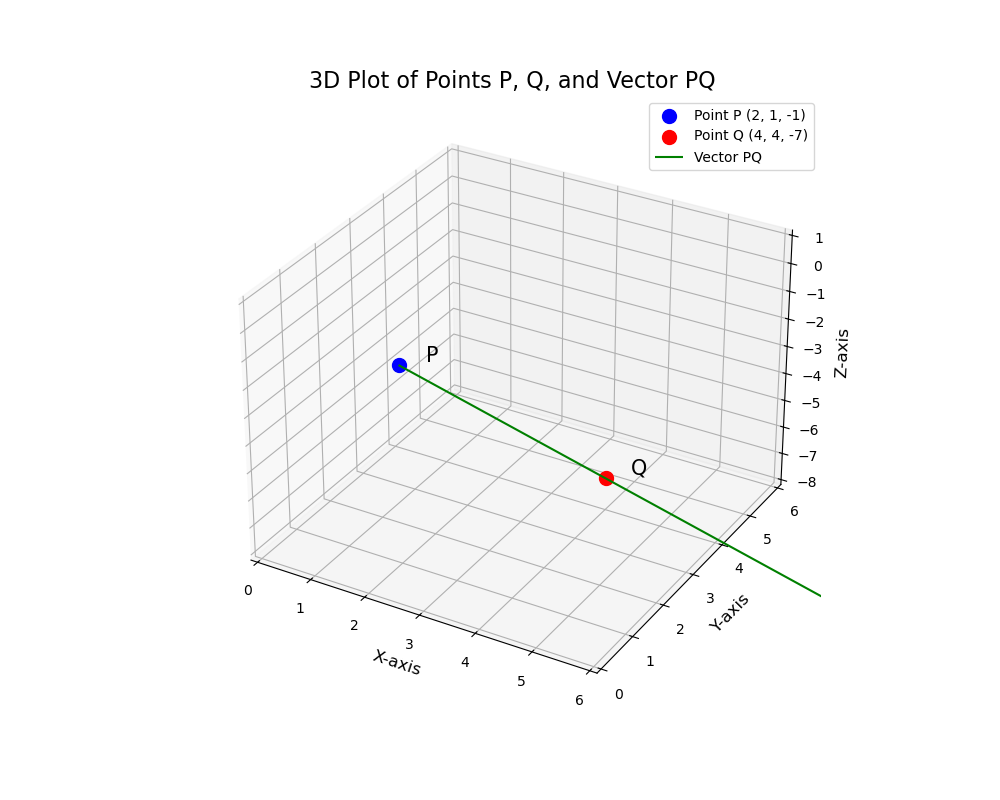
\includegraphics[width=0.63\columnwidth]{figs/fig1.png}
\end{center}
\caption{}
\label{fig:Fig.1}
\end{figure}
\end{document}




